% This is a Basic Assignment Paper but with like Code and stuff allowed in it. 

\documentclass[11pt]{article}

% Preamble

\usepackage[margin=1in]{geometry}
\usepackage{amsfonts, amsmath, amssymb}
\usepackage{fancyhdr, float, graphicx}
\usepackage[utf8]{inputenc} % Required for inputting international characters
\usepackage[T1]{fontenc} % Output font encoding for international characters
\usepackage{fouriernc} % Use the New Century Schoolbook font
\usepackage[nottoc, notlot, notlof]{tocbibind}
\usepackage{listings}
\usepackage{xcolor}
\usepackage{float}

\definecolor{codegreen}{rgb}{0,0.6,0}
\definecolor{codegray}{rgb}{0.5,0.5,0.5}
\definecolor{codepurple}{rgb}{0.58,0,0.82}
\definecolor{backcolour}{rgb}{0.95,0.95,0.92}

\lstdefinestyle{mystyle}{
    backgroundcolor=\color{backcolour},   
    commentstyle=\color{codegreen},
    keywordstyle=\color{magenta},
    numberstyle=\tiny\color{codegray},
    stringstyle=\color{codepurple},
    basicstyle=\ttfamily\footnotesize,
    breakatwhitespace=false,         
    breaklines=true,                 
    captionpos=b,                    
    keepspaces=true,                 
    numbers=left,                    
    numbersep=5pt,                  
    showspaces=false,                
    showstringspaces=false,
    showtabs=false,                  
    tabsize=2
}

\lstset{style=mystyle}

% Header and Footer
\pagestyle{fancy}
\fancyhead{}
\fancyfoot{}
\fancyhead[L]{\textit{\Large{Computer Networks Assignment 6}}}
%\fancyhead[R]{\textit{something}}
\fancyfoot[C]{\thepage}
\renewcommand{\footrulewidth}{1pt}



% Other Doc Editing
% \parindent 0ex
%\renewcommand{\baselinestretch}{1.5}

\begin{document}
	
	\begin{titlepage} 
		\centering 
		
		%---------------------------NAMES-------------------------------
		
		\huge\textsc{
			MIT World Peace University
		}\\
	
		\vspace{0.75\baselineskip} % space after Uni Name
		
		\LARGE{
			Computer Networks\\
			Second Year B. Tech, Semester 3
		}
		
		\vfill % space after Sub Name
		
		%--------------------------TITLE-------------------------------
		
		\rule{\textwidth}{1.6pt}\vspace*{-\baselineskip}\vspace*{2pt}
		\rule{\textwidth}{0.6pt}
		\vspace{0.75\baselineskip} % Whitespace above the title
		
		
		
		\huge{\textsc{
			Configuration of Static and Dynamic NAT
			}} \\
		
		
		
		\vspace{0.5\baselineskip} % Whitespace below the title
		\rule{\textwidth}{0.6pt}\vspace*{-\baselineskip}\vspace*{2.8pt}
		\rule{\textwidth}{1.6pt}
		
		\vspace{1\baselineskip} % Whitespace after the title block

		%--------------------------SUBTITLE --------------------------	
			
		\LARGE\textsc{
			Practical Report\\
			Assignment 6
		} % Subtitle or further description
		\vfill
		
		%--------------------------AUTHOR-------------------------------
		
		Prepared By
		\vspace{0.5\baselineskip} % Whitespace before the editors
		
		\Large{
			Krishnaraj Thadesar \\
			Cyber Security and Forensics\\
			Batch A1, PA 20
		}
		
		
		\vspace{0.5\baselineskip} % Whitespace below the editor list
		\today

	\end{titlepage}
	
	
\tableofcontents
\thispagestyle{empty}
\clearpage


\setcounter{page}{1}

\section{Aim and Objectives}
Implement Static and Dynamic NAT Configuration with Packet Tracer

\section{Devices}

\subsection{Devices Used}
\begin{enumerate}
	\item 1 Switch 2960 with 24 LAN Ports
	\item 2 Generic PCs
	\item 2 Routers.
	\item 1 Server. 
\end{enumerate}

\section{Cables}
\begin{enumerate}
	\item Straight LAN Cable to connect unlike Devices
	\item Crossover LAN Cable to connect like Devices
\end{enumerate}

\section{Procedure to Configure the Network}

\begin{enumerate}
	\item Create the Network as shown in the figure below.
	\item Connect the various components with respective cables. 
	\item Assign IP Addresses to the devices. 
	\item Execute Appropriate commands on the routers. 
	\item Open Web browser on PCs and Laptops and check if they are able to access the server public IP. 
\end{enumerate}

\section{Commands}

\begin{verbatim}

	FOR ROUTER 0


	Router>
	Router>enable
	Router#
	Router(config-if)#clock rate 56000
	Router#configure terminal
	Enter configuration commands, one per line.  End with CNTL/Z.
	Router(config)#interface GigabitEthernet0/0/0
	Router(config-if)#ip nat inside
	Router(config-if)#exit
	Router(config)#interface Serial0/2/0
	Router(config-if)#ip nat outside
	Router(config-if)#exit
	Router(config)#ip nat inside source static 10.0.0.1 213.20.1.1
	Router(config)#ip route 0.0.0.0 0.0.0.0 Serial0/2/0
	%Default route without gateway, if not a point-to-point interface, may impact performance
	Router(config)#
	
	
	
	FOR ROUTER 2
	
	
	
	Router>enable
	Router#
	Router(config-if)#clock rate 56000
	Router#configure terminal
	Enter configuration commands, one per line.  End with CNTL/Z.
	Router(config)#interface GigabitEthernet0/0/0
	Router(config-if)#ip nat inside
	Router(config-if)#exit
	Router(config)#interface Serial0/1/0
	Router(config-if)#ip nat outside
	Router(config-if)#exit
	Router(config)#ip nat inside source static 20.0.0.1 213.20.1.2
	Router(config)#ip nat inside source static 20.0.0.2 213.20.1.2
	Router(config)#
	Router(config)#
	Router(config)#interface GigabitEthernet0/0/0
	Router(config-if)#
	Router(config-if)#exit
	Router(config)#interface GigabitEthernet0/0/0
	Router(config-if)#
	Router(config-if)#exit
	Router(config)#ip route 0.0.0.0 0.0.0.0 Serial0/1/0
	%Default route without gateway, if not a point-to-point interface, may impact performance
	Router(config)#
\end{verbatim}

\section{Platform}
	\textbf{Operating System}: Arch Linux x86-64\\
	\textbf{IDEs or Text Editors Used}: Visual Studio Code\\
	\textbf{Programs Used}: Cisco Packet Tracer v6.0.1

\section{Output}
\begin{figure}[H]
	\centering
	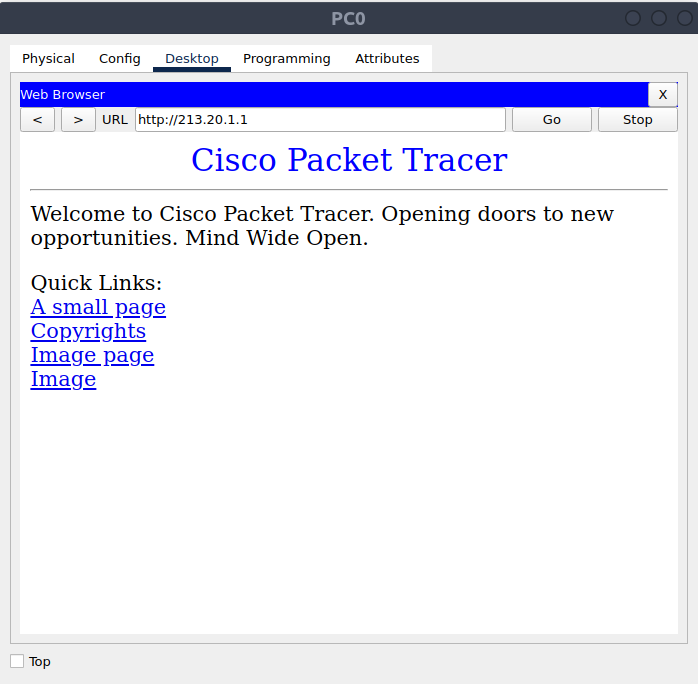
\includegraphics[scale=0.6]{../Screenshots/Natting web browser.png}
\end{figure}

\section{Connection Screenshot}


\begin{figure}[H]
	\centering
	\includegraphics[scale=0.4]{../Screenshots/Assignment_6_screenshot.png}
\end{figure}


\section{Conclusion}
Thus we have successfully configured Static and Dynamic NAT in Cisco Packet Tracer.
\end{document}

\item Serial DCE Timed Cable to connect the 2 Routers. 